\section{Containerized IOC}
Containerization is an increasingly popular method of virtualizing an application, without having to run a full-blown operating system. In current practices, containers are commonly used both in development and production environments, often together with cloud solutions. In the \gls{HEP} containers and their different applications become more and more popular. According to ~\cite{Klaus2021} the first mention of about a Docker\footnote{Docker is a set of products that use operating system level virtualization to deliver software in packages called containers.} container of the \gls{EPICS} \gls{IOC} was related to the Taurus project in 2015~\cite{taurus}. Since then containerization efforts intensified also within the \gls{FAIR} based collaborations - \gls{CBM}/\gls{MVD}~\cite{Klaus2021} and PANDA DCS~\cite{PANDA_1}.

IOC container has been prepared by the \gls{DCS} group of the \gls{PANDA} Collaboration and adjusted to the \gls{STS} needs. The latest \gls{IOC}'s image is built on EPICS R7.0.3.1 image, and it contains the most important modules and extensions i.a. asyn, autosave, calc, Modbus, and SNMP (see Figure~\ref{fig_ioc1}). By using so-called volumes (see Figure~\ref{fig_doc}) the \gls{IOC} can be used at any node with the Docker engine. Volumes are one of the mechanisms to manage application data, and it's a proper way to ensure data persistence. When a container is started, Docker loads the read-only image layer, adds a read-write layer on top of the image stack, and mounts volumes onto the container file system. Having prepared database files, st.cmd, and stream protocols if needed, an \gls{IOC} can be deployed on any node, with any operating system and processor architecture.
\begin{figure}[!h]
\centering
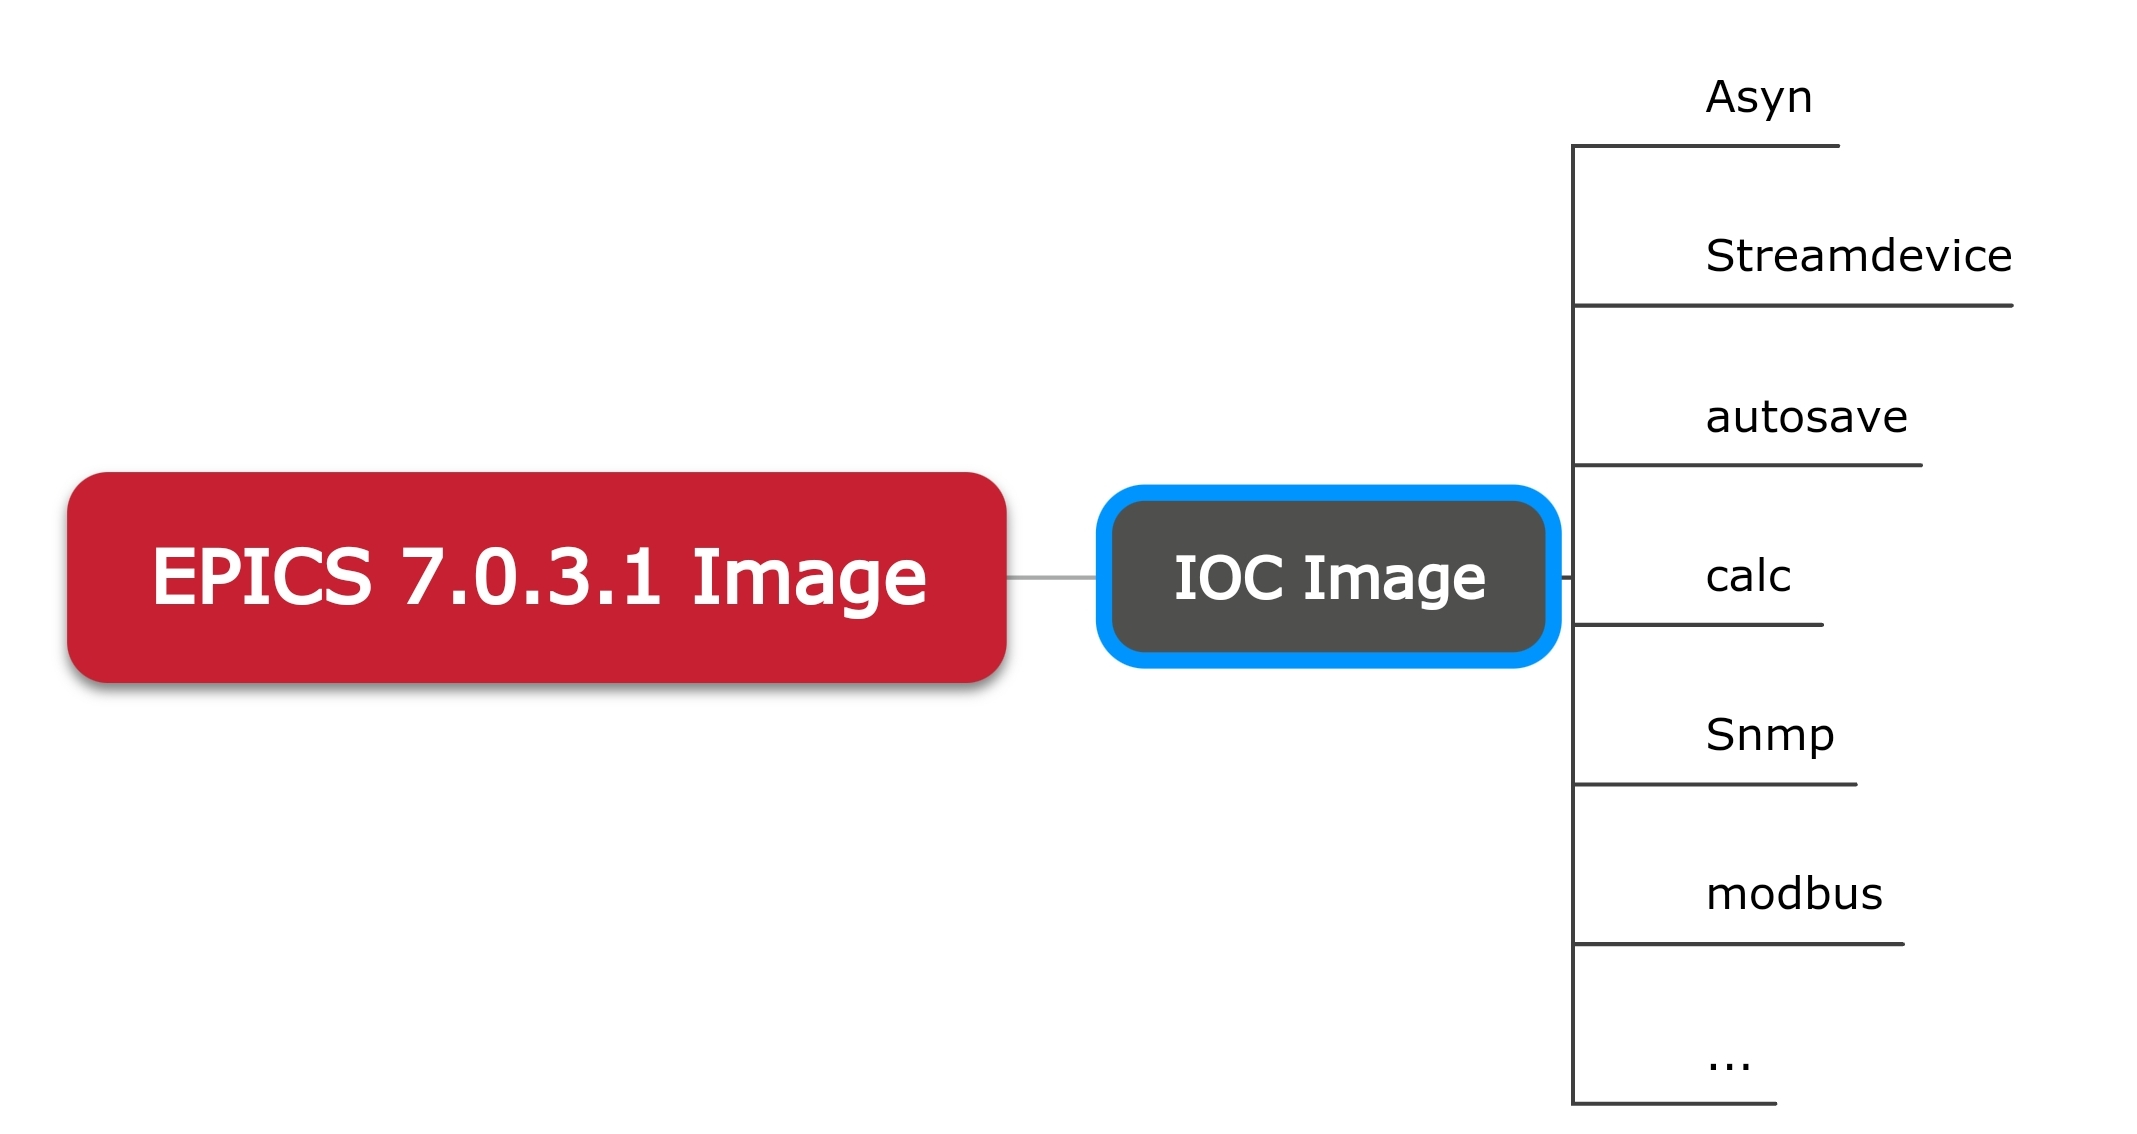
\includegraphics[width=0.7\columnwidth]{Chapter4/images/epics_ioc.jpg}
\caption{Schematic view of the EPICS 7.0.3.1 based \gls{IOC} image and the most commonly used modules.}
\label{fig_ioc1}
\end{figure}
\newpage
A general idea of a containerized \gls{EPICS} \gls{IOC} is presented in Figure~\ref{fig_doc}. Every container is assigned an IP address for every Docker network it connects to. Each network has a default subnet mask and gateway. In order to connect the \gls{IOC} with other services, the ports used by \gls{EPICS} (5064, 5065 for channel access protocol and 7064, 7065 for PVAccess) need to be exposed.  The deployed containers use the host network to communicate with each other and other nodes.
\begin{figure}[!h]
\centering
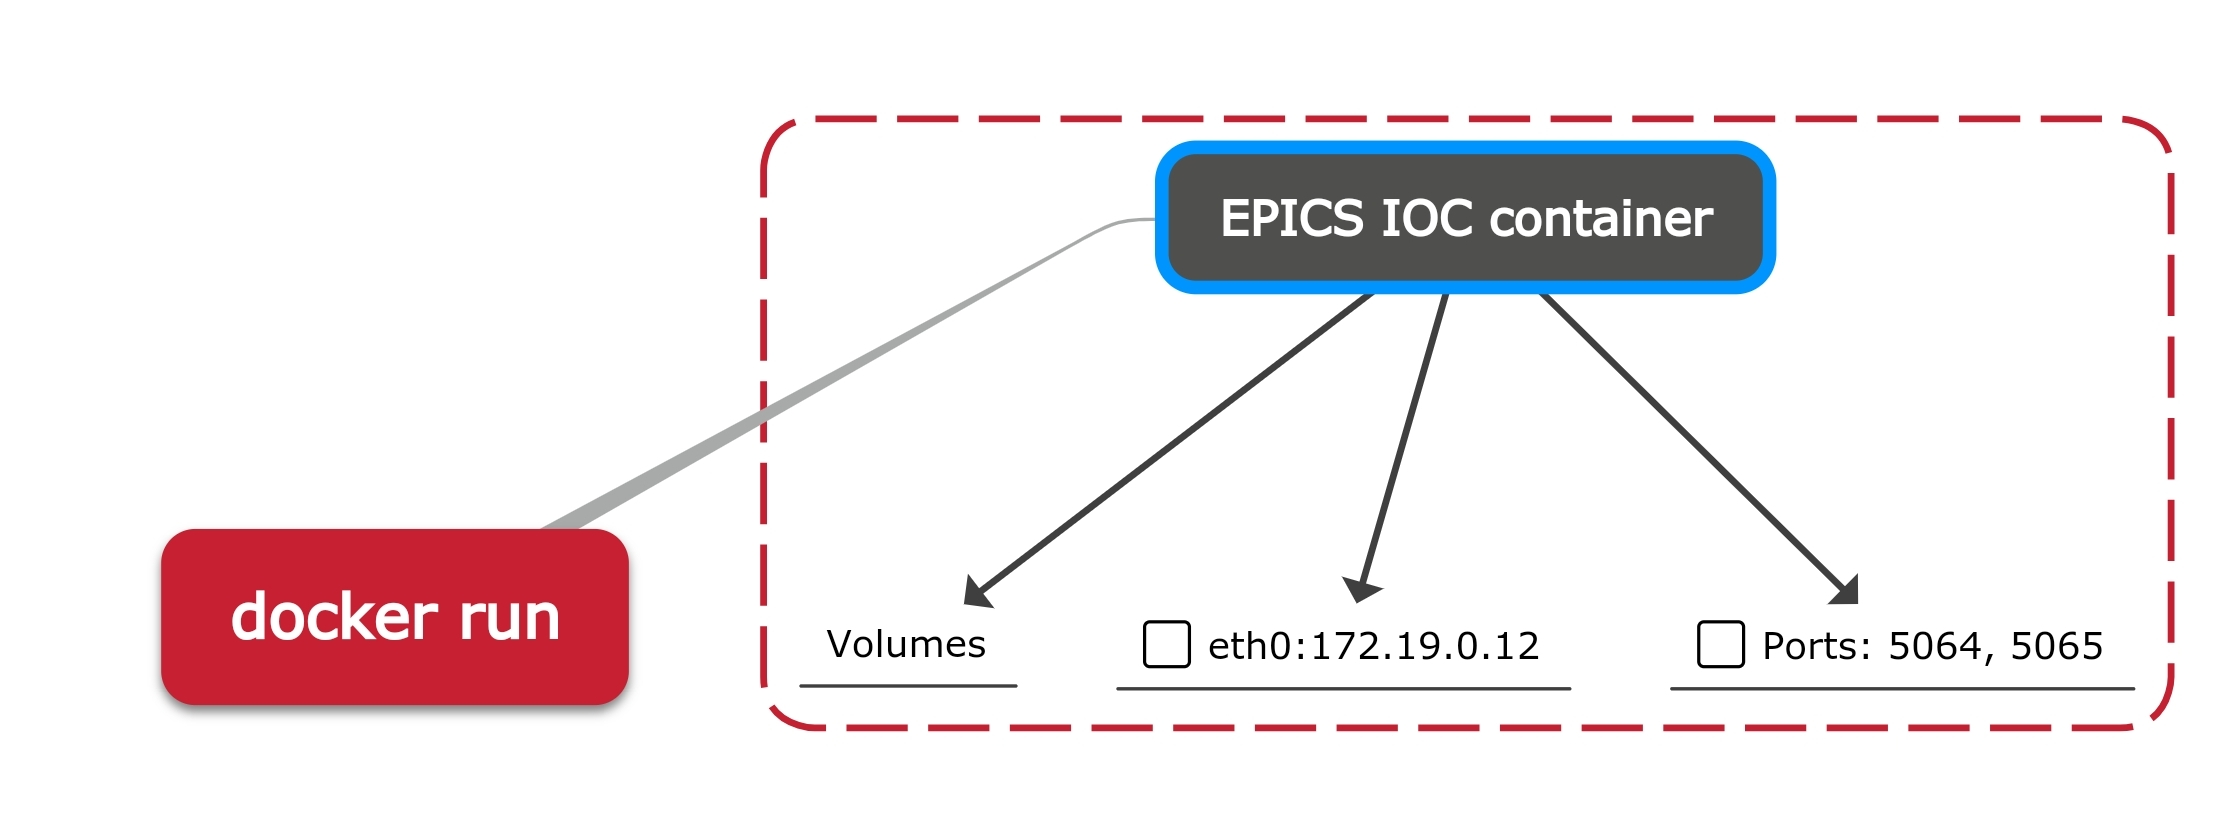
\includegraphics[width=0.75\columnwidth]{Chapter4/images/docker_run.jpg}
\caption{A general idea behind the containerization of an \gls{IOC}.}
\label{fig_doc}
\end{figure}
%\newpage
\section{Containerization platform - Docker}
Docker was chosen as the platform to prepare the images and run the containers. One of the features of docker has been considered risky for the operation of the detector/experiment, especially considering the final system. Docker-based containers run with the root privileges, therefore posing a threat to the operation of the control system. The daemon is a part of the engine that runs the containers that have full privileges not only within the container but also on the node. If a container gets compromised, it may lead to potentially disastrous scenarios, including loss of data or potential threat to the detector - e.g. killing the container. A compromised node can also endanger other nodes in the network.  Since late 2020 it's possible to run Docker daemon and containers as a non-root user. Docker daemon and containers themselves can run inside a user namespace~\cite{docker_limitations}, therefore mitigating the risk.
%\begin{figure}[!h]
%\centering
%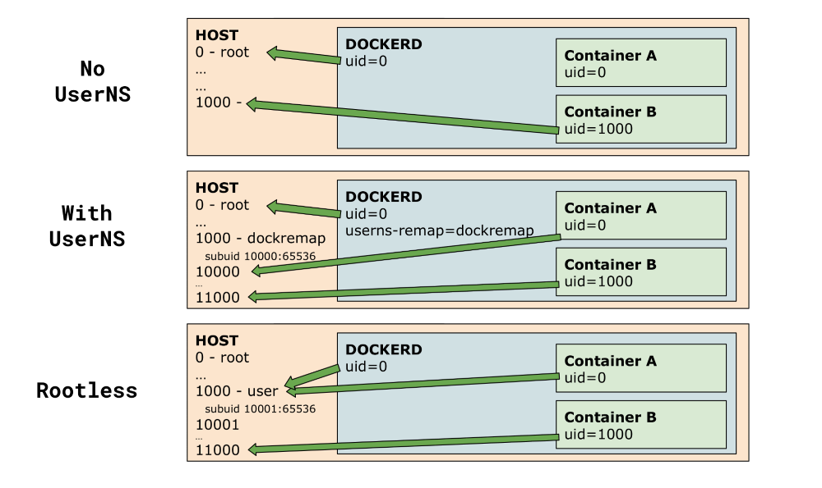
\includegraphics[width=0.8\columnwidth]{sections/images/docker.png}
%\caption{Rootless operation of the container}
%\label{fig_rootless}
%\end{figure}
 Thanks to the Open Container Initiative that defines container formats and runtimes, using different engines doesn't require many changes in the container image. There are also several alternatives to the docker engine, that allow running containers in rootless mode:
\begin{itemize}
    \item Podman~\cite{Podman} 
    \item Singularity~\cite{singularity}
\end{itemize}

For the use of containers in the final experiment, the following list of requirements must be taken into consideration:

\begin{itemize}
    \item services should be accessible only by experts, crucial services should be hidden from operators (authorization),
    \item ssh accesses to the DCS nodes should be limited by authorization plugins to avoid overloading,
    \item experiment network should be segmented based on the goals and communication between software entities clearly, defined (\gls{DCS}, \gls{SCA}),
    \item proper security context for all the services (e.g. root privileges),
    \item logging all the changes in the cluster,
    \item preventing containers from loading unwanted kernel modules,
    \item cluster, and container redundancy.
\end{itemize}


